% This file was adopted from the XML specification originally generated for
% the WISA ATLAS project. To maintain and update the specifications on a
% regular basis, the specification was added to the repo version.

\chapter{An XML file format for Cable Robots}\label{sec:XmlFileFormat}
% TEXT TAKEN FROM THE RESPECTIVE ATLAS REPORT
\section{Summery and Intent}
The following chapter contains an XML schema for the description of
cable-driven parallel robots. The structure of the XML file is introduced.
These would extend the usability if it is deemed necessary. This document
specifies an XML schema for the description of cable-driven parallel robots.
Considerable effort has been made to accommodate as many different designs and
technologies as possible in one XML structure. While considerations for the
structure stemmed from existing architectures, the only prerequisite for a
machine to be successfully defined through this XML structure is that it is a
cable-driven parallel robot; meaning that a mobile platform is positioned in
Cartesian space through controlling the length of wires attached to the
platform using winches which are attached to a fixed base.

\section{XML Schema}\label{sec:XmlFormatSpecs}
In the following, subsection a formal description for cable-driven parallel
robots using specifications of the extensible markup language (XML) is
proposed. This XML schema aims at providing a platform independent format for
exchanging of all relevant parameters. Such format enables an easy exchange of
data between different software tool, operation systems, and hardware
components.

\subsection{XML Version Definition}%
This is version~0.32 (as of 27.04.2016) of the XML schema for parallel cable
robots. A specific set of rules is needed to ensure compatibility across
multiple platforms. The format is structured such that properties of cable
robots can be broken down into distinct modules describing a specific aspect.
Individual attribute values are often of the same type of data, and there are a
limited number of data types. These data types are defined for all attributes
initially. Data types in square brackets [\ldots] indicate optional
alternatives for a type representing the same thing.  As some attributes are
optional, default values for each data type are also given.

The proposed file name extensions used by WireX is \texttt{.wcrfx}. 

\subsection{Data Types}%
The data types used to describe the technical parameters of cable robots is
limited to those described below to reduce ambiguity and facilitate effective
data transfer. The values are introduced as attributes of a XML tags.

\begin{table}
  \centering
  \caption{Data type specification}
  \label{tab:XmlDataTypeSpecs}
  \begin{tabular}{p{0.18\textwidth}p{0.18\textwidth}p{0.18\textwidth}p{0.36\textwidth}}
    \hline\hline
    Type  &  Data  &  Attribute  & Description \\
    \hline
    Int & Integer & value & Positive Integers (0, 1, 2, \ldots)\\
    Bool & Boolean Value &  N/A & Boolean "1" is TRUE; "0" FALSE.\\
    String & String & N/A & String can contain an arbitrary number of
    characters, used for labels or descriptions.\\
    String (enum) & String "enumerated" type & N/A & For this string
    accepted values are strictly defined.\\
    Scalar & Double &  value  & Using SI units scalars are single values
    of floating point arithmetic. \\
    Position Vector & Three Doubles &  x, y, z &
    Vector in 3-dimensional space to indicate a position or translation.\\
    Moment of Inertia Tensor &  Symmetric 3$\times$3 matrix (double[9]) &
    Ixx, Iyy, Izz, Ixy, Iyz, Ixz &  Describes inertia for an arbitrary axis.\\
    Rotation Matrix & Orthogonal 3$\times$3 matrix, (double[9]) &  a11, a12,
    a13, a21, a22, a23, a31, a32, a33 & Describes rotation matrix in Euclidean space.\\
    $[$Quaternion$]$ & Four Doubles & q0, q1, q2, q3 & Alternative to the
    rotation matrix to describe a rotation in Euclidian space by a normalized quaternion.\\
    $[$Axis Angle$]$ & Four Doubles & ux, uy, uz, beta & Defines rotation
    through an axis ($u_x,u_y,u_z$) and an angle ($\beta$) around this
    axis.\\
    \hline\hline
  \end{tabular}
\end{table}

All units are to be expressed using SI units (meter, kilogram, second, ampere);
regardless of common cases in literature where others (millimeters, pounds,
etc.) are prevalent.

\subsection{Default Values}%
Unless stated otherwise these are the default values for optional attributes
which are denoted by square brackets [\ldots]:
\begin{table}
  \centering
  \caption{Data type specification}
  \label{tab:XmlDefaultValues}
  \begin{tabular}{p{0.3\textwidth}p{0.18\textwidth}p{0.4\textwidth}}
    \hline\hline
    Type  &  Attribute  & Default value\\
    \hline
    Int & value & 0\\
    String & N/A  &  "" empty string (only the "NULL" terminator) \\
    Scalar & value &  0.0\\
    Position Vector & x, y, z & (0,0,0) Zero vector\\
    Moment of inertia tensor  &  Ixx, Iyy, Izz, Ixy, Iyz, Ixz & ( 0, 0, 0
    0, 0, 0)\\
    Rotation Matrix & a11, a12, a13, a21, a22, a23, a31, a32, a33 & identify matrix ( 1, 0, 0, 0, 1, 0, 0, 0, 1)\\
    $[$Quaternion$]$ & q0, q1, q2, q3 & quaternion that represents no rotation (1, 0, 0, 0)\\
    $[$Axis Angle$]$ & ux, uy, uz, beta & (0, 0, 0, 0)\\
    \hline\hline
  \end{tabular}
\end{table}

\subsection{\<User-Data> tag}%
There exists a method which allows the addition of data not specified in this
XML Schema. This is the \<User-Data> tag. This tag should not include general
information which can be expressed in any way using the XML schema. Even values
which are not explicitly stated but can be inferred (such as the number of
winches) should not be expressed here. Only information which is relevant to
individual applications specifically should be included here. A use of this tab
for regular data exchange is an indicator that the XML Schema is deficient, and
in such warrants a possible expansion of the XML Schema.

\section{General Structure}
The general structure of a file of this XML schema is organized as
shown in Fig.~\ref{fig:XmlFileFormatStructure}.
\begin{figure}[tb]
  \centering
  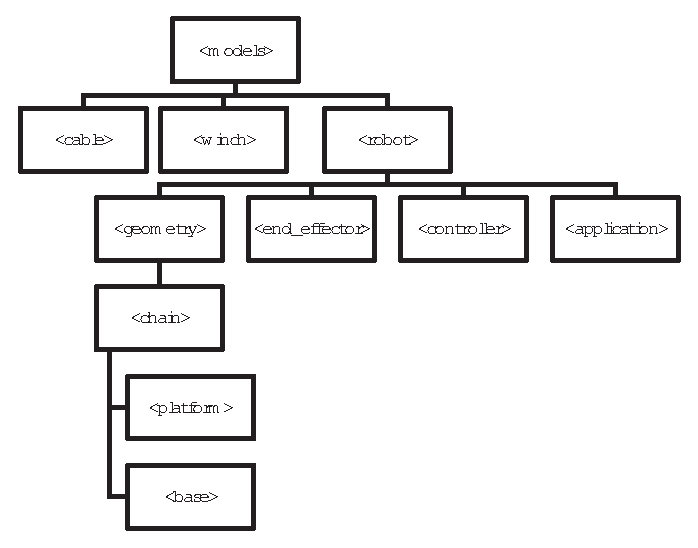
\includegraphics[width=0.8\textwidth]{XmlFileFormatStructure.eps}
  \caption{Logical structure of the XML file format}
  \label{fig:XmlFileFormatStructure}
\end{figure}
It is conceivable that XML files which only contain cable or winch information
within the \<models> tag facilitate data-exchange of these components. These
can be considered as databases of their respective kind. The contents of the
\<models> tag for a specific cable robot using one type of winch and cable
would then be as such:
\begin{verbatim}
<models>
  <robot name="IPAnema2" id="1">
    <!-- properties of the robot will be here -->
  </robot>
  <winch name="Winde1" id="1">
    <!-- properties of the winch will be here -->
  </winch>
  <cable name="SteelCable1" id="1">
    <!-- properties of the cable will be here -->
  </cable>
</models>
\end{verbatim}

The \<models> tag encompasses all the relevant data placed in the tags
\<cable>, \<winch> and \<robot> and has the following attributes:

\begin{table}
  \centering
  \caption{\<models> tag attributes}
  \label{tab:XmlModelTag}
  \begin{tabular}{p{0.3\textwidth}p{0.18\textwidth}p{0.4\textwidth}}
    \hline\hline
    Attribute & Type & Description \\
    \hline
    version & String & Version number of XML schema.\\
    \hline\hline
  \end{tabular}
\end{table}

The relevant parameters for each robot will be placed in the \<robot> tag. The
\<robot> tag contains the attributes outlined in Table~\ref{tab:XmlRobotTag}.
The attributes in the \<robot> tag hold meta-information identifying specific
robot configurations.

\begin{table}
  \centering
  \caption{\<robot> tag attributes }
  \label{tab:XmlRobotTag}
  \begin{tabular}{p{0.3\textwidth}p{0.18\textwidth}p{0.4\textwidth}}
    \hline\hline
    Attribute  & Type  &  Description \\
    \hline
    name & String & Name of the robot / robot design.\\
    id & Int & Unique identifier for this robot.\\
    \[author] & String & Name of the Author or
    Institution responsible for this robot design.\\
    \[generator] & String & Reference to the software tool used to generate this robot.\\
    \[description] & String & Description of the robot design.\\
    \[motion\_pattern] & String (enum) & Type of motion\_pattern this
    robot is able to generate. This indicates the number of
    translational (T) and rotational (R) degrees of freedom, e.g.: 3R3T
    has six d.o.f in Cartesian space. Permitted values are 1T, 2T, 3T,
    1R2T, 2R3T and 3R3T.\\
    \hline\hline
  \end{tabular}
\end{table}

The relevant parameters for each cable will be placed in the \<cable> tag. This
tag does not contain any further sub-tags as the total information relevant to
individual cables is considered relatively small. As such meta-information and
cable parameters are both described within the attributes of the \<cable> tag
presented in section~\ref{sec:XmlCable} cable parameters.

The relevant parameters for each winch will be placed in the \<winch> tag. The
\<winch> tag contains the attributes outlined in Table~\ref{tab:XmlWinchTag}.
The attributes in the \<winch> tag hold meta-information identifying specific
robot configurations.

\begin{table}
  \centering
  \caption{\<winch> tag attributes }
  \label{tab:XmlWinchTag}
  \begin{tabular}{p{0.3\textwidth}p{0.18\textwidth}p{0.4\textwidth}}
    \hline\hline
    Attribute  & Type & Description \\
    \hline
    Name & String & Name of that particular winch type.\\
    Id & Int & Unique identifier for winch type.\\
    \[creator] & String & Name of the creator or institution responsible
    for this robot design.\\
    \[description] & String & Description of winch type.\\
    \hline\hline
  \end{tabular}
\end{table}

\subsection{Cable Parameters}\label{sec:XmlCable}%
Unlike the robot parameters, cable parameters are not considered unique for a
single application. Hence cable types are defined separately in within the
cable tag. These types can be grouped to provide a library of cables which can
be part of a specific robot, or an independent database with only cable types.
The \<cable> tag contains the attributes outlined in
Tab.~\ref{tab:XmlCableTag}. The attributes in the \<cable> tag hold
meta-information identifying cable types and specific cable parameters.

\begin{table}
  \centering
  \caption{\<cable> tag attributes}
  \label{tab:XmlCableTag}
  \begin{tabular}{p{0.3\textwidth}p{0.18\textwidth}p{0.4\textwidth}}
    \hline\hline
    Attribute  & Type  &  Description \\
    \hline
    name & String & Name of that particular cable.\\
    id & Int & Unique identifier for cable type.\\
    \[radius] & Scalar & Radius of the cable \[m].\\
    \[weight] & Scalar & Specific weight of the cable \[kg/m].\\
    \[damping] & Scalar & Specific damping\\
    \[elasticity]& Scalar & Specific elasticity of the cable \[1/N].\\
    \[breaking\_load]& Scalar & Breaking load in \[N]\\
    \[minimum\_load] & Scalar & Minimum load in \[N]\\
    \[max\_length] & Scalar & Maximum cable length in \[m]\\
    \hline\hline
  \end{tabular}
\end{table}

\subsection{Winch}%
Winches are complex assemblies with many different possible layouts. The focus
in this tag will be on parameters directly affecting the cable robot. Similarly
to the cable parameters the winch parameters are combined to only contain
information of specific winches, so that they can be grouped as a database, or
applied to several robot geometries.

Winch parameters are described in the \<winch> tag. Due to the complexity the
physical parameters are grouped in relevant sub-tags within the \<winch> tag.

\begin{table}
  \centering
  \caption{Tags contained within the \<winch> tag}
  \label{tab:XmlWinchTagOverview}
  \begin{tabular}{p{0.3\textwidth}p{0.18\textwidth}p{0.4\textwidth}}
    \hline\hline
    Tag  & Attributes  &  Description \\
    \hline
    \<cable> & In Tab.~\ref{tab:XmlCableTag2} & Relevant winch parameters in relation to the cables.\\
    \<motor> & In Tab.~\ref{tab:XmlMotorTag} & Parameters of the motor drive.\\
    \<drum> & In Tab.~\ref{tab:XmlDrumTag} & Parameters of the cable drum.\\
    \<guiding\_limit> & In Tab.~\ref{tab:XmlGuidinglimitTag} & Description of the possible cable direction vectors from the point of exit\\
    \<linear\_drive> & In Tab.~\ref{tab:XmlLineardriveTag} & Parameters of a linear drive (if used)\\
    \<anchoring> & In Tab.~\ref{tab:XmlAnchoringTag} & Physical description of the anchoring mechanisms (for evaluating attachment to frame)\\
    \hline\hline
  \end{tabular}
\end{table}

Each tag defined in Table~\ref{tab:XmlWinchTagOverview} contains further
attributes to include winch parameters. These attributes listed in the
following tables.

The \<cable> tag contains the attributes listed in Tab.~\ref{tab:XmlCableTag2}.
These attributes contain specific winch parameters relating to the cable
actuated by the winch.

\begin{table}
  \centering
  \caption{\<cable> tag attributes}
  \label{tab:XmlCableTag2}
  \begin{tabular}{p{0.3\textwidth}p{0.18\textwidth}p{0.4\textwidth}}
    \hline\hline
    Attribute & Type & Description \\
    \hline
    nr\_cables & Int & Number of cables per winch. \\
    transmission\_ratio & Scalar & The ratio between motor turns and cable length.\footnote{This value is the best estimate, and theoretically could be calculated with enough information on the winch geometry, but as it is deemed essential to cable robot manipulation it is explicitly stated here. It is conceivable that some winches may have a non-inear transmission ratio; but as of yet the XML Schema does not accommodate for this. Should the need exist a separate tag within the \<winch> tag is likely.} \\
    \[f\_max] & Scalar & Maximum tension force exerted on the cable \[N].\\
    \[f\_hold\_max] & Scalar & Maximum holding force \[N].\\
    \[string\_orientation] & String & Nominal direction of the cable in $\Re^3$\\
    \[dl\_max] & Scalar & Maximum cable length variation \[m]\\
    \[l\_min]& Scalar & Minimum cable length \[m].\\
    \[max\_velocity] & Scalar & Maximum cable velocity \[m/s].\\
    \[max\_acceleration] & Scalar & Maximum cable acceleration \[m/s$^2$].\\
    \[max\_jerk] & Scalar& Maximum cable jerk \[m/s$^3$].\\
    \[position\_sensor\_accuracy] & Scalar & Accuracy of the position sensors \[m].\\
    \[force\_sensor\_accuracy]& Scalar & Accuracy of the force sensors \[N].\\
    \[spring\_constant] & Scalar & Spring constant of the winch \[m/N].\\
    \[length\_offset] & Scalar & Length offset for the cable length \[m].\\
    \hline\hline
  \end{tabular}
\end{table}

The \<motor> tag contains the attributes listed in Tab.~\ref{tab:XmlMotorTag}.
These attributes contain specific winch parameters relating to the motor
specifications.

\begin{table}
  \centering
  \caption{\<motor> tag attributes}
  \label{tab:XmlMotorTag}
  \begin{tabular}{p{0.3\textwidth}p{0.18\textwidth}p{0.4\textwidth}}
    \hline\hline
    Attribute & Type  &  Description \\
    \hline
    motor\_type & String & Type of motors (i.e. servo, stepper, etc.)\\
    \[inertia] & Scalar & Motor inertia in \[kg m$^2$]\\
    \[mass] & Scalar & Motor mass in [kg]\\
    \[max\_power]& Scalar & Motor power [W]\\
    \[angular\_velocity] & Scalar & Angular velocity of motor [rads/s]\\
    \[angular\_acceleration] & Scalar & Angular acceleration of motor[rad/s$^2$]\\
    \[gear\_ratio] & Scalar & Gear ratio of the drive train\\
    \hline\hline
  \end{tabular}
\end{table}

The \<drum> tag contains the attributes listed in Table~\ref{tab:XmlDrumTag}.
These attributes contain specific winch parameters relating to the cable drum
of the winch. All drum parameters are optional parameters.
\begin{table}
  \centering
  \caption{\<drum> tag attributes}
  \label{tab:XmlDrumTag}
  \begin{tabular}{p{0.3\textwidth}p{0.18\textwidth}p{0.4\textwidth}}
    \hline\hline
    Attribute & Type  &  Description \\
    \hline
    \[r\_drum]  &  Scalar & Radius of the drum in [m]\\
    \[l\_drum]  &  Scalar & Length of the drum in [m]\\
    \[nr\_groove] &Scalar & Number of turns of the cable groove on the drum\\
    \[groove\_depth] & Scalar & Groove depth in [m]\\
    \[dfriction]& Scalar & Dynamic friction of drum on mount [N]\\
    \[sfriction]& Scalar & Static friction of drum on mount [N]\\
    \[backlash] & Scalar & Backlash [m]\\
    \hline\hline
  \end{tabular}
\end{table}

The \<guidinglimit> tag contains the attributes listed in
Tab.~\ref{tab:XmlGuidinglimitTag}. These attributes describe the possible cable
feed directions of the winch geometry.

\begin{table}
  \centering
  \caption{\<guidinglimit> tag attributes}
  \label{tab:XmlGuidinglimitTag}
  \begin{tabular}{p{0.3\textwidth}p{0.18\textwidth}p{0.4\textwidth}}
    \hline\hline
    Attribute & Type & Description \\
    \hline
    \[aperture] & Scalar & Angle of the aperture of to define a cone of possible cable orientations in [rad]\\
    \[cone\_offset] & Position Vector & Apex point offset from point $A_i$.\\
    \hline\hline
  \end{tabular}
\end{table}

The \<lineardrive> tag contains the attributes listed in
Tab~\ref{tab:XmlLineardriveTag}. These attributes describe cable winch if a
drum is replaced by a linear drive.

\begin{table}
  \centering
  \caption{\<lineardrive> tag attributes}
  \label{tab:XmlLineardriveTag}
  \begin{tabular}{p{0.3\textwidth}p{0.18\textwidth}p{0.4\textwidth}}
    \hline\hline
    Attribute & Type & Description \\
    \hline
    \[nr\_pulleys] & Int & Number of pulleys\\
    \[min\_length] & Scalar & Minimal length \[m]\\
    \[max\_length] & Scalar & Maximum length \[m]\\
    \[inertia\_moment] & Scalar & Moment of intertia of the entire assembly \[kg\ m$^2$]\\
    \[dfriction] & Scalar & Dynamic friction \[N]\\
    \[sfriction] & Scalar & Satic friction \[N]\\
    \hline\hline
  \end{tabular}
\end{table}

The \<anchoring> tag contains the attributes listed in
Tab.~\ref{tab:XmlAnchoringTag}. These attributes describe cable winch if a drum
is replaced by a linear drive

\begin{table}
  \centering
  \caption{\<anchoring> tag attributes}
  \label{tab:XmlAnchoringTag}
  \begin{tabular}{p{0.3\textwidth}p{0.18\textwidth}p{0.4\textwidth}}
    \hline\hline
    Attribute & Type & Description \\
    \hline
    \[type] & String & A description of the type of anchoring\\
    \[max\_force] & Scalar & Maximum force permitted for this anchoring \[N]\\
    \[acting\_moment] & Position Vector & Vector defining the moment exerted by the winch in \[m]\\
    \hline\hline
  \end{tabular}
\end{table}

\subsection{Geometry and Layout}%
Layout and geometry of the cable robot are described in the \<geometry> tag.
This describes the physical layout which is unique to each robot even for exact
copies of functionality and parts will always contain positioning errors which
can be reflected here. For every winch-platform pair (or cable connection to
the platform) one \<chain> tag is added. This chain describes the geometrical
positions of these kinematic links and mostly governs the robots properties.
The number of cables is represented by the number of \<chain> tags within the
\<geometry> tag. Each chain has its own identification number in order to pair
the right winch and cable types to one specific chain. The \<chain> tag
contains the attributes outlined in Tab.~\ref{tab:XmlChainTag}. The attributes
in the \<chain> tag hold meta-information identifying a chain and pairing the
correct cable/winch type.
%
\begin{table}
  \centering
  \caption{\<chain> tag attributes}
  \label{tab:XmlChainTag}
  \begin{tabular}{p{0.3\textwidth}p{0.18\textwidth}p{0.4\textwidth}}
    \hline\hline
    Attribute & Type & Description \\
    \hline
    id & Int & Unique identifier for this chain beginning with 1\\
    \[winch\_type] & String & Identification of a specific winch which is defined using a \<winch> tag.\\
    \[cable\_type] & String & Identification of a specific cable which is defined using a \<cable> tag.\\
    \hline\hline
  \end{tabular}
\end{table}

The geometric parameters are defined through the tags described in
Tab.~\ref{tab:XmlChainSubTag}.

\begin{table}
  \centering
  \caption{Tags within the \<chain> tag}
  \label{tab:XmlChainSubTag}
  \begin{tabular}{p{0.3\textwidth}p{0.18\textwidth}p{0.4\textwidth}}
    \hline\hline
    Tag & Attribute & Description \\
    \hline
    \<base> & Position Vector & Vector identifying the characteristic exit point of the cable defined in the world coordinate system $\mathcal K_0$. (In the case of a winch with pulley kinematics this would be point $A_i$) in [m]\\
    \<base> & Rotation Matrix or Quaternion or Axis Angle & Winch orientation: When using pulley kinematics the direction of the rotation axis and the reference plane for the determination of the angles.\\
    \<base> & Radius="Scalar" & Radius of the Pulley in [m];\\
    \<platform> & Position Vector & Vector identifying the characteristic end point of the cable on the platform. Defined in the coordinate system of the platform ($\mathcal K_p$)\\
    \<platform> & Rotation Matrix or Quaternion or Axis Angle & Orientation of the coordinate system $\mathcal K_{Bi}$ which describes the characteristics of the cable end point. Defines a normal cable direction.\\
    \hline\hline
  \end{tabular}
\end{table}

A typical robot geometry can be defined as follows:
\begin{verbatim}
<models>
  <robot name="IPAnema2">
    <geometry>
      <!-- A Simple Winch-->
      <chain id=1>
        <base x="1.0" y="2.0" z="0.0"/>
        <platform x="0.1" y="0.05" z="0.0"/>
      </chain>
      <!-- A Winch with orientation -->
      <chain id=2>
        <base x="-1.0" y="2.0" z="0.0" q0="1" q1="0" q2="0" q3="0"/>
        <platform x="-0.1" y="0.05" z="0.0"/>
      </chain>
      <!-- More chain tags follow to describe further connections -->
    </geometry>
  </robot>
  <!-- More robots,  winches, or cable parameters can be placed here -->
</models>
\end{verbatim}
The example defines a cable robot named "IPAnema2" with two winches which is of
cause of little practical use. The first winch is place at $a_1=[1.0, 2.0
,0.0]^T$ and the cable is connected to the mobile platform at $b_1=[0.1,
0.05, 0.0]^T$. The reference coordinate system for the winches is not rotated
with respect to the world coordinate frame since the respective attributes in
the \<base> and \<platform> tags is left out and the default values apply. For
the second winch ($a_2=[-1.0, 2.0, 0.0]^T, b_2=[-0.1, 0.05,
0.0]^T$) an orientation is described for the winches. Here the quaternion
$Q=[1,0,0,0]$ is used to the orientation of the winch.

\subsection{Mobile Platform}%
The \<end\_effector> tag is used to describe the attributes of the mobile
platform. It is to be placed in the \<robot> tag. The \<end\_effector> tag
contains the tags and attributes described in Tab.\ref{tab:XmlEndeffectorTag}.
The attributes in the \<end\_effector> tag holds meta-information of the
platform and specific physical parameters. The geometric information for the
platform's anchor points are stored in the \<chain> tag.

\begin{table}
  \centering
  \caption{Tags within the \<end\_effector> tag}
  \label{tab:XmlEndeffectorTag}
  \begin{tabular}{p{0.3\textwidth}p{0.18\textwidth}p{0.4\textwidth}}
    \hline\hline
    Attribute & Type  &  Description \\
    \hline
    \<end\_effector> & name=\-"String" & Name of the platform\\
    \<end\_effector> & description=\-"String" & Description of platform\\
    \<end\_effector> & mass=\-"double" & Mass in \[kg]\\
    \<end\_effector> & swing\_angle=\-"double" & Permitted cable swing angle \[rad]\\
    \<inertia> & Moment of Inertia Tensor & Platform moment of inertia tensor \[kg\ m$^2$]\\
    \<centre\_of\_gravity> & Position Vector & Center of gravity of the platform define in the platform coordinate system ($\mathcal K_p$) [m$^3$]\\
    \hline\hline
  \end{tabular}
\end{table}

Within the \<end\_effector> tag there are the attributes "name", "description",
"mass", and "swing\_angle", in addition to two tags \<inertia> and
\<centre\_of\_gravity>  which contain more complex data structures inertia
tensor and position vector.

\subsection{Controller}%
The \<controller> tag is used to describe the attributes of the control loop of
the cable robot. It is to be placed in the \<robot> -tag. The \<controller>-tag
contains the attributes described in Tab.~\ref{tab:XmlController}. The
attributes in the \<controller> tag holds meta-information of the controller
and specific physical parameters.

\begin{table}
  \centering
  \caption{\<controller> tag attributes}
  \label{tab:XmlController}
  \begin{tabular}{p{0.3\textwidth}p{0.18\textwidth}p{0.4\textwidth}}
    \hline\hline
    Attribute & Type & Description \\
    \hline
    ipo\_clock & Scalar & interpolator cycle time \[s]\\
    dim\_x & Int & Dimensions of controller variables\\
    delay\_time & Scalar & Time Constant of the delay time in \[s]\\
    time\_discrete & Bool & Indicator whether the control is in discrete time steps "1" or continuous "0".\\
    \hline\hline
  \end{tabular}
\end{table}

The number of inputs and outputs for the controller is defined (similar to with
the \<chain> tag) through the number of tags and is not explicitly stated.
Attributes of the tags  \<input\_port> and \<output\_port> are described in
Tab.~\ref{tab:XmlInputTag} and Tab.~\ref{tab:XmlOutputTag} respectively. The
attributes in of these tags hold meta-information of the input/output.

\begin{table}
  \centering
  \caption{\<input\_port> tag attributes}
  \label{tab:XmlInputTag}
  \begin{tabular}{p{0.3\textwidth}p{0.18\textwidth}p{0.4\textwidth}}
    \hline\hline
    Attribute & Type & Description \\
    \hline
    type & String & Type of input; "enumerated" string with the following values:
    \{lin\_position, rot\_position, lin\_velocity, rot\_velocity, lin\_acceleration, rot\_acceleration, force, torque\}\\
    chain\_id & Int & Identifier of the relevant chain id\\
    \hline\hline
  \end{tabular}
\end{table}


The \<output\_port>-tag and the \<input\_port>-tag, have the same structure.

\begin{table}
  \centering
  \caption{\<output\_port> tag attributes}
  \label{tab:XmlInputTag}
  \begin{tabular}{p{0.3\textwidth}p{0.18\textwidth}p{0.4\textwidth}}
    \hline\hline
    Attribute & Type & Description \\
    \hline
    type & String & Type of output; "enumerated" string with the following values:
    \{lin\_position, rot\_position, lin\_velocity, rot\_velocity, lin\_acceleration, rot\_acceleration, force, torque\}\\
    chain\_id & Int & Identifier of the relevant chain id\\
    \hline\hline
  \end{tabular}
\end{table}

\subsection{Application}
The \<application> tag is used to describe the attributes of the control loop
of the cable robot. It is to be placed in the \<robot> tag. The
\<application>-tag contains the attributes described in
Tab.~\ref{tab:XmlApplicationTag}. The attributes in the \<application> tag
holds meta-information of the specific application for which the cable robot is
design and physical parameters.

\begin{table}
  \centering
  \caption{\<application> tag attributes}
  \label{tab:XmlApplicationTag}
  \begin{tabular}{p{0.3\textwidth}p{0.18\textwidth}p{0.4\textwidth}}
    \hline\hline
    Attribute & Type & Description \\
    \hline
    name & String & Name of the application\\
    \[description] & String & Further description of the application\\
    \[load\_mass] & Scalar & max. mass acting on the platform \[N]\\
    \[load\_moment] & Scalar & max. moment acting on the platform \[Nm]\\
    \[min\_cable\_load] & Scalar & min. acceptable cable load \[N]\\
    \[max\_cable\_load] & Scalar & max. acceptable cable load \[N]\\
    \hline\hline
  \end{tabular}
\end{table}
